\section{Iteration \#3 -- $kd$-Tree Exploration}

Some index structures that reduce the dimensionality of points via a hashing function degenerate to semi-sequential scan when processing the two scientific datasets. To find an index structure which performs well on these scientific datasets, this iteration turns an entirely different type of structure which is based on a \textit{hierarchical} decomposition of space. An implementation of the point $kd$-Tree is evaluated alongside the best performing hash-based approaches from the previous iterations.

\subsection{Point $kd$-Tree}

The $kd$-Tree variant described in Section \ref{sec:kd-tree-chosen} was implemented, which shall be referred to as the \textbf{Point $kd$-Tree}. Each node is represented as a C-struct which stores a single point as well as pointers to its children. Every node is allocated using a call to \texttt{malloc()}, which allocates enough memory on the heap to store the node. This means each node may reside in different areas of the heap, resulting in fragmented memory.

\subsection{Performance Timings}

\begin{figure}
	\makebox[\textwidth][c]{%
		\begin{subfloat}[\texttt{insert}\label{fig:perf3-dimensionality-insert}]{%
			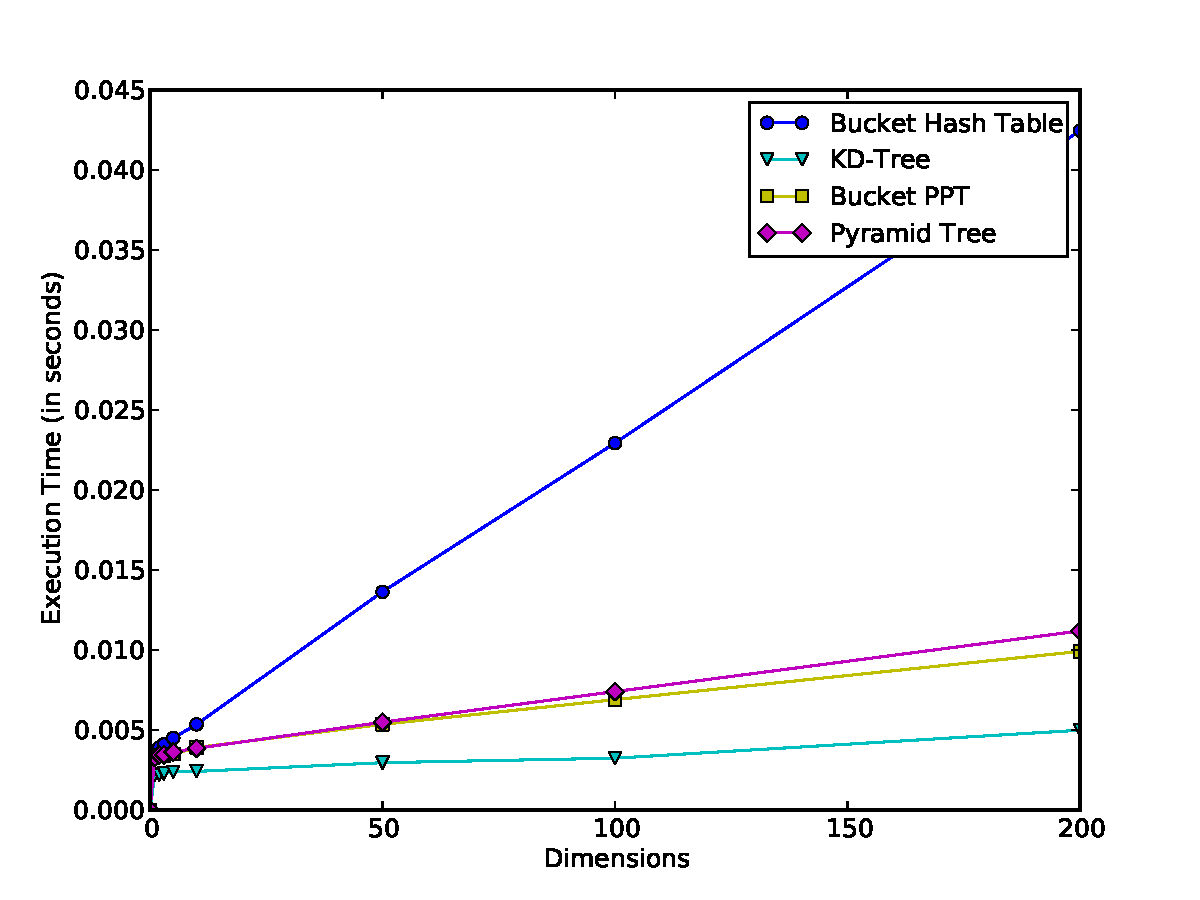
\includegraphics[scale=0.5]{figures/performance_analysis/iteration_3/randuniform_insert.pdf}
		}
		\end{subfloat}
		\begin{subfloat}[\texttt{delete}\label{fig:perf3-dimensionality-remove}]{%
			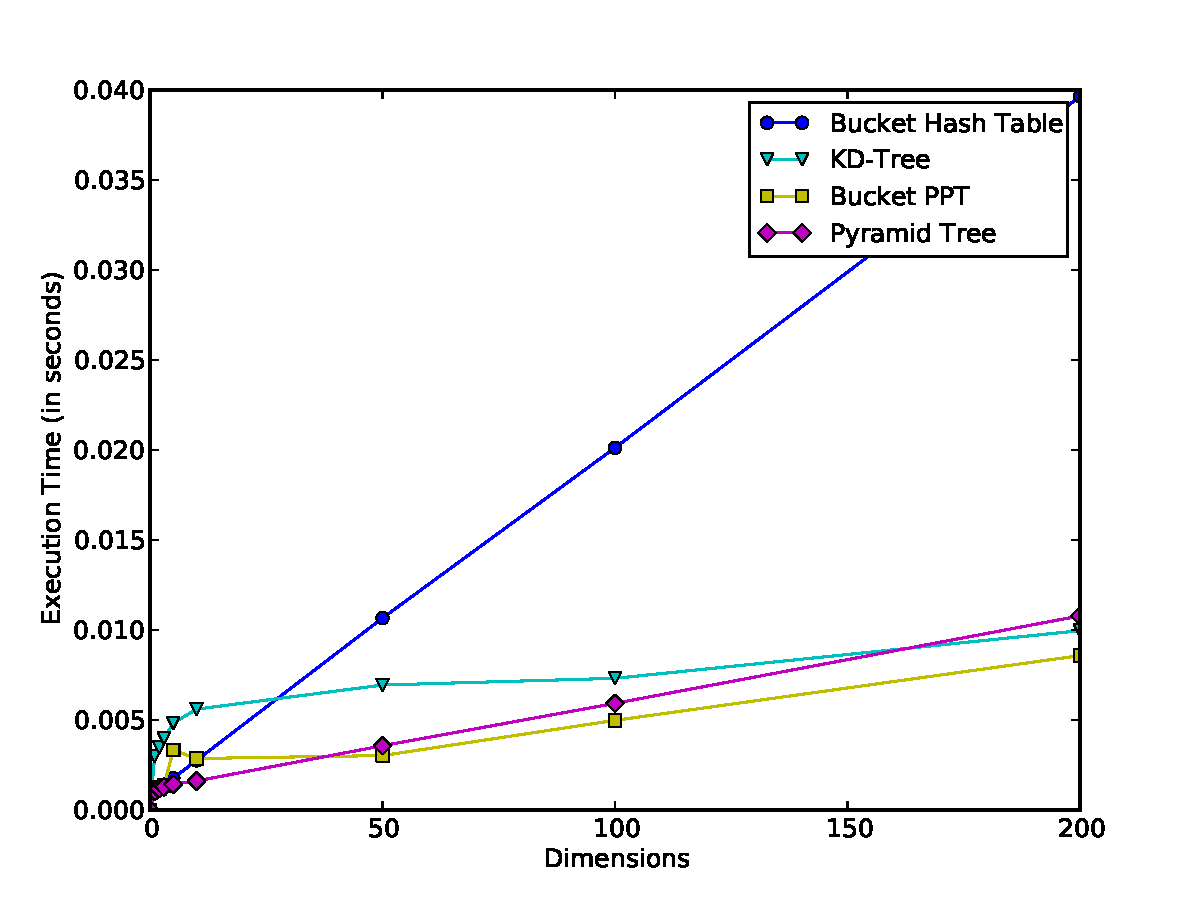
\includegraphics[scale=0.5]{figures/performance_analysis/iteration_3/randuniform_delete.pdf}
		}
		\end{subfloat}
	}%

	\caption{Index Structure Performance With Respect To Dimensionality (10,000 Points from Uniform Distribution Synthetic Dataset)}
	\label{fig:perf3-dimensionality}
\end{figure}

\begin{figure}
	\makebox[\textwidth][c]{%
		\begin{subfloat}[\texttt{insert}\label{fig:perf3-size-insert}]{%
			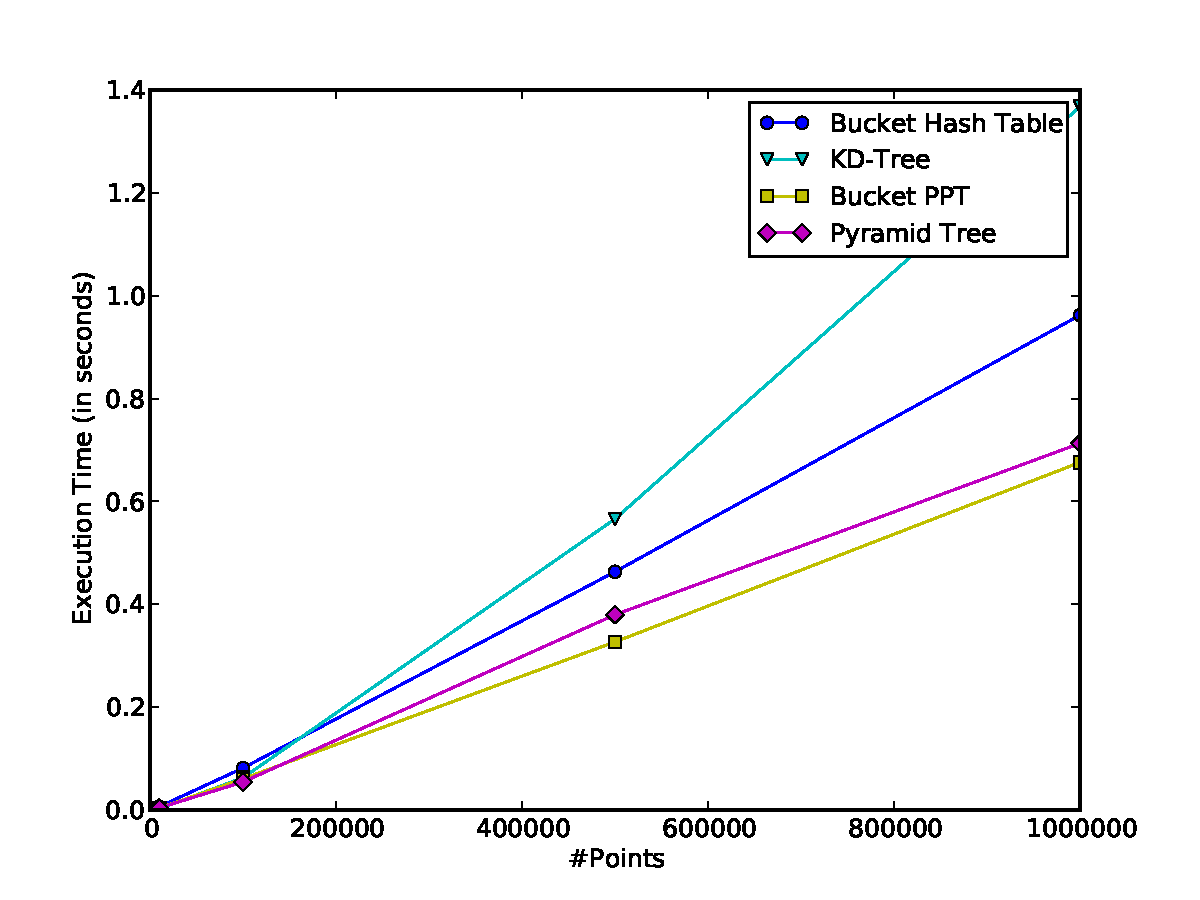
\includegraphics[scale=0.5]{figures/performance_analysis/iteration_3/sizevary_insert.pdf}
		}
		\end{subfloat}
		\begin{subfloat}[\texttt{delete}\label{fig:perf3-size-remove}]{%
			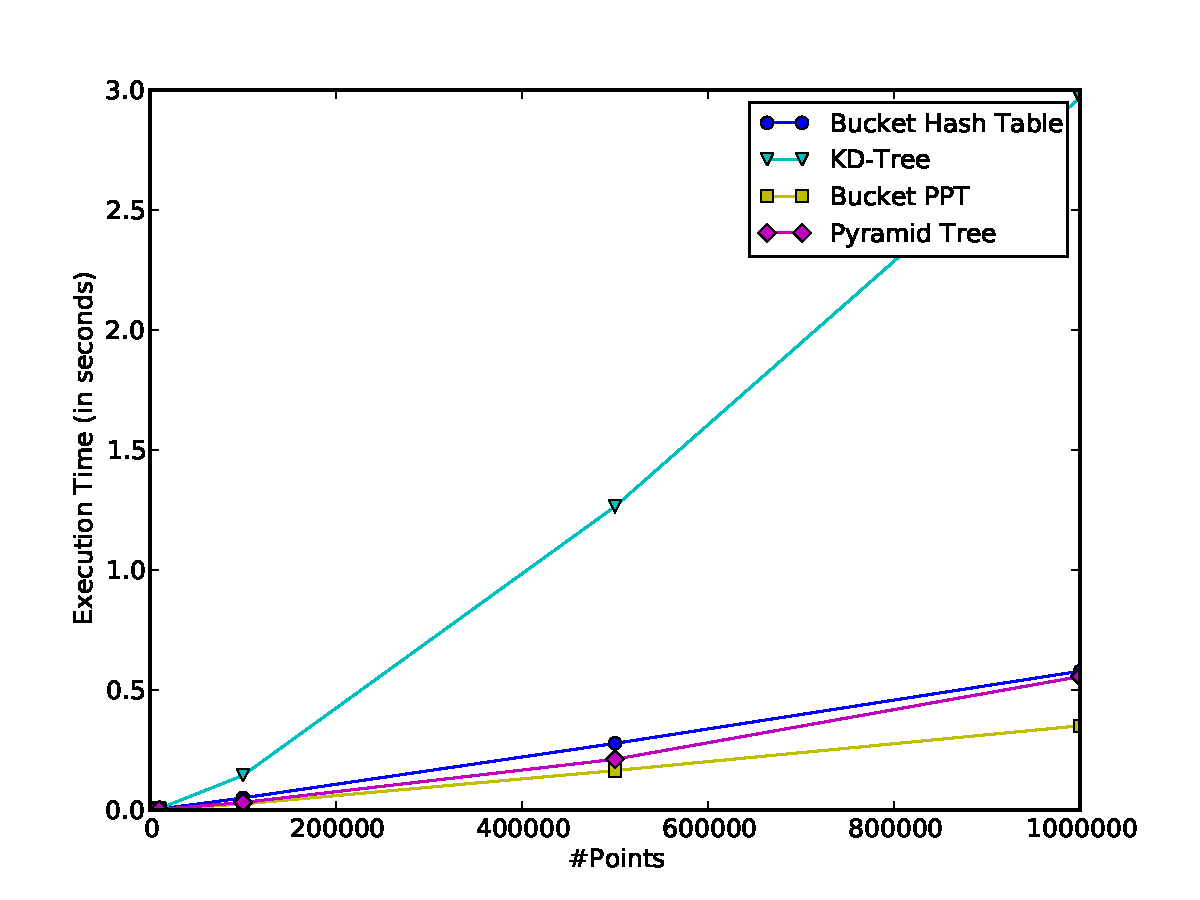
\includegraphics[scale=0.5]{figures/performance_analysis/iteration_3/sizevary_delete.pdf}
		}
		\end{subfloat}
	}%

	\caption{Index Structure Performance With Respect To Dataset Size (10,000 Points from Uniform Distribution Synthetic Dataset)}
	\label{fig:perf3-size}
\end{figure}

Tables containing the total execution times of all three operations of each structure for all synthetic datasets is available in Appendix \ref{sec:appendix-perf3}. Plots with dimension against execution time are shown for \texttt{insert} and \texttt{delete} in Figure \ref{fig:perf3-dimensionality} when processing random points from a uniform distribution.

In general, as $d$ increases the speed of the hash-based structures decreases faster than the $kd$-Tree. For insertion, the $kd$-Tree consistently outperforms the hash-based structures. For deletion, the $kd$-Tree is initially slower but as $d$ increases it starts to beat the hash-based structures. This is most likely because each hashing function takes $O(d)$ time. The $kd$-Tree does not require such a function to begin the search and as such, is more resilient to higher-dimensional search for point queries.

The Bucket Hash Table results in lower bucket size at the cost of a more expensive hashing function. Despite having the same complexity, the Pseudo-Pyramid Tree and Pyramid Tree hash functions require less computation (i.e. the constant factor is lower). Since these two structures also result in low average bucket size for synthetic data, they are faster than the Bucket Hash Table for synthetic data. Figure \ref{fig:perf3-dimensionality} illustrates this by showing that the growth in execution time of Bucket Hash Table is the fastest. 

The execution times between the Pyramid Tree and the Pseudo-Pyramid Tree is very small, but the latter structure is consistently faster. Table \ref{tab:perf2-bucket-stats} in Section \ref{sec:bucket-stats} shows that the Pseudo-Pyramid Tree results in lower bucket size for random points generated from a uniform distribution. This combined with the fact the Pseudo-Pyramid Tree function requires slightly less computation makes it faster than the Pyramid Tree.

Execution times for the 16 dimension dataset of varying size is shown in Figure \ref{fig:perf1-size}. While the $kd$-Tree performs faster when $d$ is increased, the increase in speed becomes negligible as more points are inserted into the structures. This is especially the case with \texttt{delete}, where execution time grows much faster.

As long as the average bucket size tends to one, the speed of the hash-based structures is higher than the $kd$-Tree. Since all three hash-based structures have low average bucket size for the synthetic data, the relative performance of the structures depends on the hashing function itself. Since the Pseudo-Pyramid Tree has the cheapest hashing function, it is the fastest structure for the synthetic datasets.

\subsection{Real Datasets}

\begin{table}
	\centering
	\makebox[\textwidth][c]{%
		\begin{tabular}{|r|r|l|l|l|}
			\hline
			\multicolumn{2}{|c}{} & \multicolumn{3}{|c|}{\textbf{Dataset}} \\
			\hline
			\textbf{Structure} & \textbf{Operation} & \textbf{Astrophysics} & \textbf{Hurricane Isabel} & \textbf{Armadillo Mesh} \\
			\hline
			\multirow{4}{*}{Bucket Hash Table} & Delete & 0.191339 & 0.248544 & 0.102674 \\
				& Insert & 0.360452 & 0.419106 & 0.11828 \\
				& Point Query & 0.172516 & 0.222288 & 0.0811833 \\
			\hline
			\multirow{4}{*}{$kd$-Tree} & Delete & 68.9612 & 578.798 & 0.91045 \\
				& Insert & 0.663231 & 0.434781 & 0.384241 \\
				& Point Query & 0.639265 & 0.408527 &  0.374425 \\
			\hline
			\multirow{4}{*}{Bucket PPT} & Delete & 82.908 & 71.006 & 0.160532 \\
				& Insert & 81.231 & 69.401 & 0.126938 \\
				& Point Query & 70.4391 & 69.3368 & 0.0956872 \\
			\hline
			\multirow{4}{*}{Pyramid Tree} & Delete & 60.8105 & 64.9182 & 0.164531 \\
				& Insert & 65.0126 & 69.5751 & 0.192165 \\
				& Point Query & 60.0216 & 69.4891 & 0.134481 \\
			\hline
		\end{tabular}
	}%
	\caption{Total Execution Time (in seconds) of Each Operation on Sampled Real Datasets}
	\label{tab:perf3-real}
\end{table}

Table \ref{tab:perf3-real} shows the runtime of each operation on sampled real datasets. Bucket Hash Table is consistently the fastest structure for all operations and data because its average bucket size is always close to one. Again, the Pseudo-Pyramid Tree and Pyramid Tree degenerate to semi-sequential on the two scientific datasets, with the Pyramid Tree performing slightly better than the Pseudo-Pyramid Tree on the astrophysics dataset.

The $kd$-Tree is over one hundred times faster than the Pseudo-Pyramid and Pyramid Trees for the scientific datasets for \texttt{insert} and point queries. However, the structure processes these datasets slower than the synthetic data or armadillo mesh. $kd$-Tree's \texttt{delete} operation is also the slowest of all the structures, taking over 500 seconds to individually delete all the points from the hurricane dataset.

\subsection{Impact of $kd$-Tree Balance}

The performance timings in the previous section show that the $kd$-tree becomes slower with particular datasets. Despite the $kd$-Tree storing the same number of points in each of the real datasets, the performance is different. The speed of processing 500,000 points from the astrophysics or hurricane Isabel datasets is much slower than the armadillo mesh or the synthetic datasets. 

The cause of this is most likely the \textit{balance} of the tree. Skewed datasets are known to affect the balance of spatial decomposition trees, resulting in longer paths from the root node to the leaves. To investigate this further, the \textit{balance factor} of the point $kd$-tree, when storing 500,000 points from three synthetic and three real datasets has been measured. The balance factor is defined as the \textit{average} length of a path from the root to a leaf \cite{kdtree-v-bdtree}. A lower balance factor means the $kd$-Tree has to visit less nodes on average when performing a point query, so queries will generally be faster. A $kd$-Tree is balanced when its balance factor is $\log_2 n$. When $n = 500,000$, the best possible balance factor is $\log_2 (500,000) \approx 19$.

The \textit{exact match query cost}, used to evaluate $kd$-tree variations by Dandamudi and Sorenson \cite{kdtree-v-bdtree}, represents the average number of points visited in the tree for a point query. Higher exact match query cost means the tree has to do more work on average to find a point, making the structure slower.

\begin{table}
	\centering
	\makebox[\textwidth][c]{%
		\begin{tabular}{|l|l|l|l|}
			\hline
			\multicolumn{1}{|c|}{\textbf{Dataset}} & \centrespecialcell{\textbf{Balance} \\ \textbf{Factor}} & \centrespecialcell{\textbf{Max Path} \\ \textbf{Length}} & \centrespecialcell{\textbf{Exact Match} \\ \textbf{Query Cost}} \\
			\hline
			\leftspecialcell{Random 10D Points \\ (Uniform Distribution)} & 24.8285 & 47 & 24.4968 \\
			\leftspecialcell{Random 10D Points \\ (Skewed Distribution)} & 24.9092 & 44 & 24.5714 \\
			\leftspecialcell{Random 10D Points \\ (Clustered Distribution)} & 30.3362 & 57 & 29.9911 \\
			Astrophysics & 32.405 & 120 & 29.7373 \\
			Hurricane Isabel & 47.7236 & 123 & 40.5602 \\
			\hline
		\end{tabular}
	}%
	\caption{Point $kd$-Tree Balance Factor and Exact Match Query Cost with 500,000 Points from Various Datasets}
	\label{tab:kdtree-balance-factor}
\end{table}

The balance factor clearly increases as $n$ is increased, so the concern here is how its affected by data distribution. Table \ref{tab:kdtree-balance-factor} contains the balance factor and maximum path length from the root to a leaf when the point $kd$-Tree is storing points from datasets with different distributions. It also contains the exact match query cost of querying all the points stored in the $kd$-Tree. 

The table shows that the exact match query cost increases as the balance factor does and thus, the average amount of work required to perform a point query. While the $kd$-tree does not degenerate when processing datasets with skew, these results show that these datasets do affect the structure's overall performance. For this reason, many variants of the $kd$-Tree have been developed with the goal of reducing the balance factor, such as the BD-Tree \cite{kdtree-v-bdtree} and fair split tree\cite{fair-split-tree}. However, it is beyond the scope of this document to explore these variants here.

\subsection{Summary}

This iteration showed that the point $kd$-tree, even with no attempts to further optimise the structure, significantly outperformed the Pseudo-Pyramid Tree and Pyramid Tree. The point $kd$-Tree is slower than the Bucket Hash Table, especially with individual point deletion, but it is more resilient to floating point inaccuracy as it does not rely on a potentially inaccurate hashing function. The timing data from this iteration results in the following observations:
\begin{enumerate}[noitemsep]
	\item if a \textit{reliable} hashing function that produces an average bucket size very close to one can be found, then a structure which is faster than the point $kd$-Tree for point queries can be constructed
	\item the point $kd$-Tree is affected by point distribution as shown by the increased balance factor and average point query cost when storing the two scientific datasets
	\item individual point deletion from point $kd$-Trees is the slower than every hash-based structure implemented
\end{enumerate}

